\documentclass[t,10pt,xcolor={dvipsnames}]{beamer}
\usetheme[
%%% option passed to the outer theme
%    progressstyle=fixedCircCnt,   % fixedCircCnt, movingCircCnt (moving is deault)
  ]{Feather}

%%% light theme
%% Change back color
%\setbeamercolor{background canvas}{bg=white}
%% Change the bar colors:
%\setbeamercolor{Feather}{fg=red!50!gray,bg=red!50!black}
%% Change the color of the structural elements:
%\setbeamercolor{structure}{fg=red!50!black}
%% Change the frame title text color:
%\setbeamercolor{frametitle}{fg=black!5}
%% Change the normal text colors:
%\setbeamercolor{normal text}{fg=black!75,bg=white}
%% Change the block title colors
%\setbeamercolor{block title}{use=Feather,bg=Feather.fg, fg=black!90} 

%% dark theme
% Change back color
\setbeamercolor{background canvas}{bg=black}
% Change the bar colors:
\setbeamercolor{Feather}{fg=red!25!black,bg=red!40!black}
% Change the color of the structural elements:
\setbeamercolor{structure}{fg=red!60!white}
% Change the frame title text color:
\setbeamercolor{frametitle}{fg=white!5}
% Change the normal text colors:
\setbeamercolor{normal text}{fg=white!75,bg=black}
% Change the block title colors
\setbeamercolor{block title}{use=Feather,bg=Feather.fg, fg=white!90} 

% Change the logo in the upper right circle:
\renewcommand{\logofile}{images/logo_irphe.png} 
%% This is an image that comes with the LaTeX installation
% Adjust scale of the logo w.r.t. the circle; default is 0.875
\renewcommand{\logoscale}{0.8}

% Change the background image on the title and final page.
% It stretches to fill the entire frame!
\renewcommand{\backgroundfile}{images/background.pdf}
\renewcommand{\backgroundopacity}{0.0}

%-------------------------------------------------------
% INCLUDE PACKAGES
%-------------------------------------------------------

\usepackage[utf8]{inputenc}
\usepackage[english]{babel}
\usepackage{multicol}

\usepackage{ulem} % sout
\usepackage{cancel}

%-------------------------------------------------------
% DEFFINING AND REDEFINING COMMANDS
%-------------------------------------------------------

% colored hyperlinks
\newcommand{\chref}[2]{
  \href{#1}{{\usebeamercolor[bg]{Feather}#2}}
}

\graphicspath{{schemes/}}

%-------------------------------------------------------
% PRESENTATION SPECIFIC PACKAGES AND DEFINITIONS
%-------------------------------------------------------

\usepackage{tikz}
\usetikzlibrary{math}
\usepackage{pgf}
\usepackage{pgfplots, pgfplotstable}
\usepgfplotslibrary{groupplots}
\usepgfplotslibrary{fillbetween}
\pgfplotsset{compat=newest}

%%%%% visible on command

\tikzset{
	invisible/.style={opacity=0},
	visible on/.style={alt={#1{}{invisible}}},
	alt/.code args={<#1>#2#3}{%
		\alt<#1>{\pgfkeysalso{#2}}{\pgfkeysalso{#3}} % \pgfkeysalso doesn't change the path
		},
}

%%%% Colors (used for the plots)

\definecolor{colorplot0}{rgb}{1.0,0.5,0.5}
\definecolor{colorplot1}{rgb}{0.5,1.0,0.5}
\definecolor{colorplot2}{rgb}{0.5,0.5,1.0}

%%%% Notations

\newcommand{\Direction}{\hat{\vec{z}}}
\newcommand{\SwimmingDirection}{\hat{\vec{p}}}

%-------------------------------------------------------
% INFORMATION IN THE TITLE PAGE
%-------------------------------------------------------

\title[Beamer presentation template used by Rémi Monthiller during his PhD] % [] is optional - is placed on the bottom of the sidebar on every slide
{ % is placed on the title page
	\textbf{\LARGE Based on the amazing Feather Beamer Theme by Lilyana Vankova}\\
}

\subtitle[]
{
}

\author[Rémi Monthiller]
{   
	\vspace{-20pt}
	\large \textbf{Rémi Monthiller},$^1$\\ 
	\vspace{5pt}
	\normalsize \textbf{Second Author,$^1$ Third Author,$^2$ Forth Author,$^1$ and Last Author$^1$}\\
	\vspace{5pt}
	\small $^1$Aix Marseille Univ, CNRS, Centrale Marseille, IRPHE, Marseille, France\\
	$^2$Some, Other, Stuff
}

\institute[IRPHE]
{%
}

\date{}
%\date{June 10, 2021}
%\date{\today}

%-------------------------------------------------------
% THE BODY OF THE PRESENTATION
%-------------------------------------------------------

\begin{document}

%-------------------------------------------------------
% FRAME TITLE
%-------------------------------------------------------

{\1% % this is the name of the PDF file for the background
\begin{frame}[plain,noframenumbering] % the plain option removes the header from the title page, noframenumbering removes the numbering of this frame only
  \titlepage % call the title page information from above
\end{frame}}

%-------------------------------------------------------
% FRAME 1
%-------------------------------------------------------

\begin{frame}{A simple slide example}{With a image included}
	\pause
	\vspace{10pt}
	\centering
	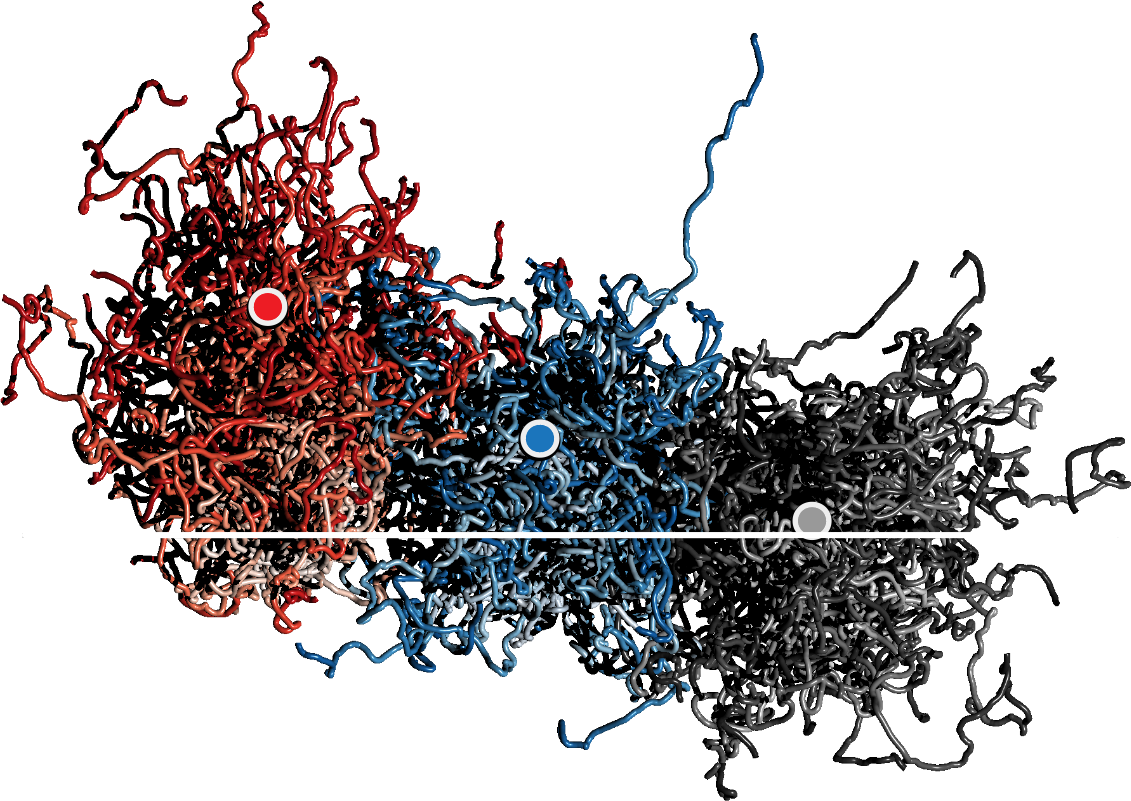
\includegraphics[width=0.7\textwidth]{schemes/trajectories.png}

	\vskip0pt plus 1filll % Used to align things with the bottom of the slide
	
	\visible<2->{\scriptsize Bali, Balo et al. (2021),}\visible<3->{and Another et al. (2019).}
	\vspace{10pt}
\end{frame}

%-------------------------------------------------------
% FRAME 2
%-------------------------------------------------------

\begin{frame}{A two columns slide}{Using pgfplots}
	\pause
	\vspace{40pt}
	\centering
	\begin{columns}[c]
		\column{.5\textwidth}
		\centering
		\begin{tikzpicture}
	% gain as a function of the free parameter $\alpha$
	\begin{axis} [
		axis on top,
		%%% size
		width=\textwidth,
		%height=\textwidth,
		%%% y
		%ymin=0,
		%ymax=1,
		ylabel={$y$},
		%ymode=log,
		%%% x
		xlabel=$x$,
		%xmin=0,
		%xmax=1,
		%%% legend
		legend cell align=left,
		legend pos = north west,
		legend style={
			draw=none, 
			fill=none, 
			xshift=2pt, 
			/tikz/every even column/.append style={column sep=0pt}
		},
	]
		\node[anchor=center] at (axis cs:3,1) {annotation};
		%% JHTDB
		%%% 95 CI
		\addplot[name path=A, draw=none, forget plot] table [
			x index=0,
			y expr={\thisrowno{1} + \thisrowno{2}},
			col sep=comma, 
			comment chars=\#,
			unbounded coords=discard,
		]{data/amazing_data.csv};
		\addplot[name path=B, draw=none, forget plot] table [
			x index=0, 
			y expr={\thisrowno{1} - \thisrowno{2}},
			col sep=comma, 
			comment chars=\#,
			unbounded coords=discard,
		]{data/amazing_data.csv};
		\addplot[colorplot0, opacity=0.4, forget plot] fill between[of=A and B];
		%%% average
		\addplot
		[
		color=colorplot0,
		opacity=1.0,
		only marks,
		%solid,
		mark=square*,
		]
		table[
			x index=0, 
			y index=1,
			col sep=comma, 
			comment chars=\#,
			unbounded coords=discard,
		]{data/amazing_data.csv};
		\addlegendentry{$E$};
	\end{axis}
\end{tikzpicture}


		\column<3->{.5\textwidth}
		\centering
		\begin{tikzpicture}
	% gain as a function of the free parameter $\alpha$
	\begin{axis} [
		axis on top,
		%%% size
		width=\textwidth,
		%height=\textwidth,
		%%% y
		%ymin=0,
		%ymax=1,
		ylabel={$y$},
		%ymode=log,
		%%% x
		xlabel=$x$,
		%xmin=0,
		%xmax=1,
		%%% legend
		legend cell align=left,
		legend pos = north west,
		legend style={
			draw=none, 
			fill=none, 
			xshift=2pt, 
			/tikz/every even column/.append style={column sep=0pt}
		},
	]
		%%% average
		\addplot
		[
			color=colorplot0,
			domain=0:4,
			samples=100,
			visible on=<3->,
			thick
		] {
			x^2
		};
		\addlegendentry{$x^2$};
		%%% average
		\addplot
		[
			color=colorplot1,
			domain=0:4,
			samples=100,
			visible on=<4->,
			thick
		] {
			sqrt(x)
		};
		\addlegendentry{$\sqrt{x}$};
		%%% average
		\addplot
		[
			color=colorplot2,
			domain=0:4,
			samples=100,
			visible on=<5->,
			thick
		] {
			5 + x
		};
			\addlegendentry{$5 + x$};
	\end{axis}
\end{tikzpicture}

	\end{columns}

	\vskip0pt plus 1filll
	
	\visible<6->{
		\begin{itemize}
			\item Amazing conclusion of the slide $E = mc^2$.
		\end{itemize}
	}
	\vspace{30pt}
\end{frame}

%-------------------------------------------------------
% FRAME 3
%-------------------------------------------------------

\begin{frame}{Some more}{Lists and tikz "animation"}
	\vspace{10pt}
	\begin{center}
		Amazing question?
		\vspace{10pt}
		\begin{columns}[c]
			\column{.5\textwidth}
			\begin{itemize}
				\item<1-> Yes!
				\item<2-> No...
				\item<3-> Hum... Maybe?
			\end{itemize}

			\column<2->{.5\textwidth}
			\begin{tikzpicture}
				\visible<3->{
					\draw[->] (-1,-0.5) -- (-1,0.5) node[midway, anchor=east]{$\Direction$};
				}
				\visible<2->{
					\node[inner sep=0pt] (copepod) at (1.5,0) {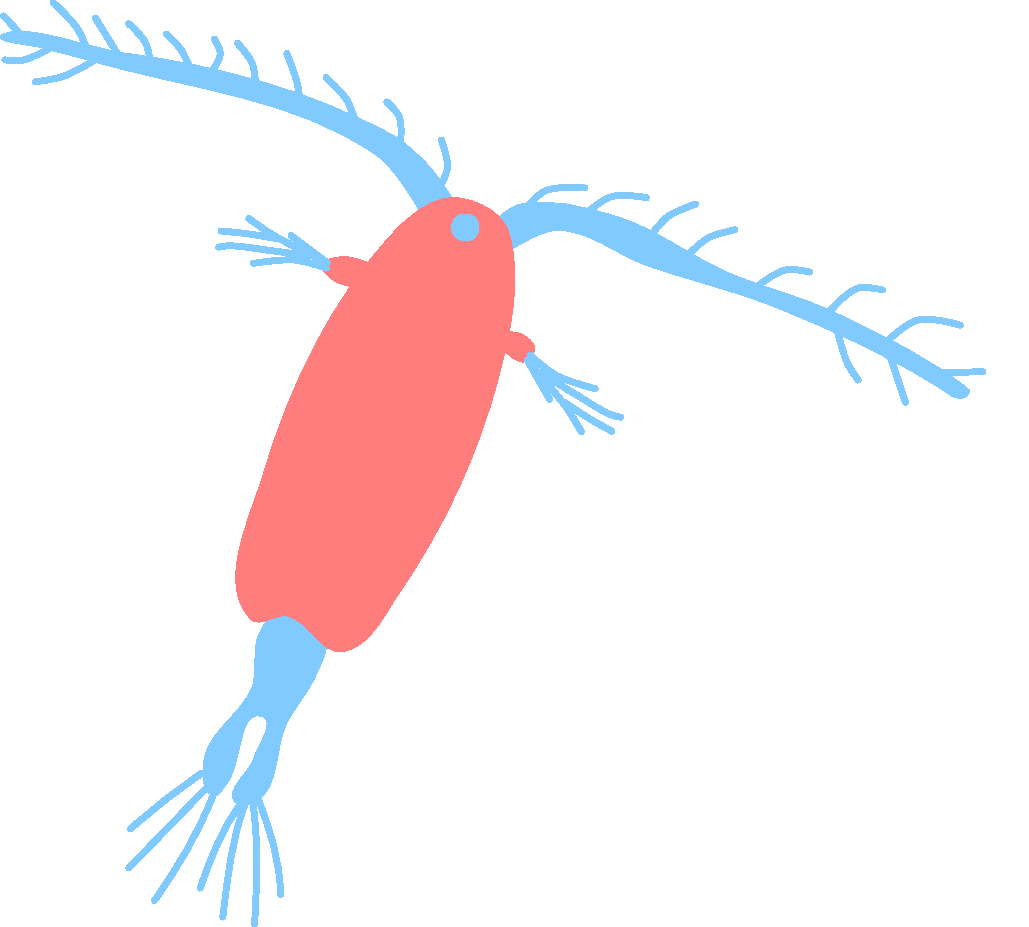
\includegraphics[width=0.36\textwidth]{schemes/copepod.pdf}};
				}
				\visible<4->{
					\draw[->] (1.5,0.5) -- (2,1) node[anchor=west]{$\SwimmingDirection$ = ?};
				}
			\end{tikzpicture}
		\end{columns}
	\end{center}
\end{frame}

%-------------------------------------------------------
% FRAME 4
%-------------------------------------------------------

\begin{frame}{A slide with a video}{Click on the figure to run the video}
	\vspace{60pt}
	\centering

	\href{run:videos/jhtdb.mp4}{
\includegraphics[width=0.5\textwidth]{images/jhtdb.pdf}}
			
	\scriptsize Rendering by Gudmundur Adalsteinsson.
\end{frame}

%-------------------------------------------------------
% FRAME CONCLUSION
%-------------------------------------------------------

\begin{frame}{Conclusion}
	\vspace{20pt}
	\begin{center}
		This is an amazing conclusion.
		\vspace{10pt}
		\begin{itemize}
			\setlength\itemsep{10pt}
			\item<2-> Pine
			\item<3-> Apple
				\begin{itemize}
					\item<5-> Red Apple
				\end{itemize}
			\item<4-> Pineapple
		\end{itemize}
	\end{center}
\end{frame}

%-------------------------------------------------------
% BACKUP FRAME 1
%-------------------------------------------------------

\begin{frame}[noframenumbering]{A backup slide}{With no frame numbering}
	\centering
	\vspace{20pt}
	Some amazing backup slide content.
\end{frame}

\end{document}
